\documentclass[a4paper,10pt]{article}
\usepackage[utf8]{inputenc}
\usepackage{tikz}
\usetikzlibrary{arrows,decorations.pathmorphing,backgrounds,positioning,fit,petri}
\renewcommand*{\familydefault}{\sfdefault}

\tikzset{forestyle/.style = {rectangle, thick, minimum width = 5cm, minimum height = 0.5cm, text width = 4.5cm, outer sep = 1mm},  
	pre/.style={<-, shorten <=1pt, >=stealth, ultra thick},
	extend/.style={<-,dashed, shorten <=1pt, >=stealth, ultra thick}}


\begin{document}

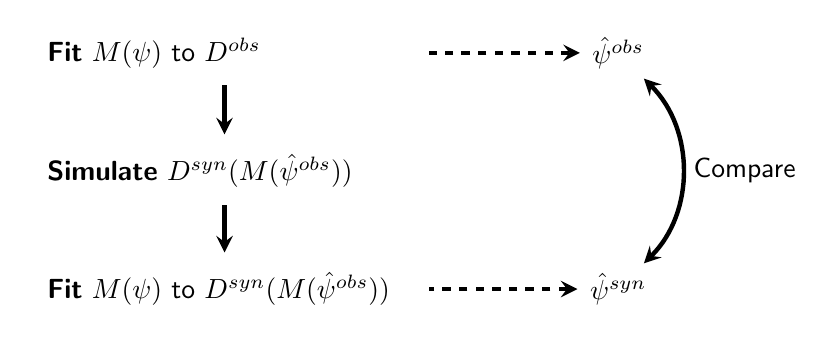
\begin{tikzpicture}

 \node (step1) at (0,0) [forestyle] {\textbf{Fit} $M(\psi)$ to $D^{obs}$};
 \node (estimated) at (5,0)  {$\hat{\psi}^{obs}$}
  edge [extend] (step1);
 
 \node (step2) at (0, -1.5) [forestyle] {\textbf{Simulate} $D^{syn}(M(\hat{\psi}^{obs}))$}
  edge [pre] (step1);
 
 \node (step3) at (0, -3) [forestyle] {\textbf{Fit} $M(\psi)$ to $D^{syn}(M(\hat{\psi}^{obs}))$}
  edge [pre] (step2);;
 \node (synthetic) at (5,-3) {$\hat{\psi}^{syn}$}
  edge [extend] (step3)
  edge [<->, ultra thick, bend right = 45, >=stealth] node[auto,swap] (compare) {Compare} (estimated);

 
\end{tikzpicture}

\end{document}
